\documentclass[a4paper, 11pt]{article}
\usepackage[margin=0.5in]{geometry}
\usepackage{framed}
\usepackage{graphicx}
\usepackage{xcolor}
\usepackage{blindtext}
\usepackage{xcolor}
\usepackage{mdframed}
\usepackage{indentfirst}
\usepackage{graphicx}
\usepackage{subcaption}
\usepackage{hyperref}
%\usepackage{txfonts}
\usepackage{amsmath}
\usepackage{titling}
\usepackage{titlesec}
\usepackage[brazil]{babel}
\definecolor{LightGray}{gray}{0.97}
\usepackage{minted}
\usepackage{xcolor} % to access the named colour LightGray

\setminted[fortran]{  framesep=2mm,
  baselinestretch=1.2,
  bgcolor=LightGray,
  fontsize=\footnotesize,
  linenos}

\titleformat{\section}{\normalfont\Large\bfseries}{\thesection}{1em}{}[\titlerule] 
\titleformat{\subsection}{\normalfont\large\bfseries}{\thesubsection}{1em}{} 
% \renewcommand\thesubsection{\Alph{subsection}}
\graphicspath{ {./graficos/} }

\begin{document}
\noindent
\large\textbf{Autor:} Jefter Santiago \hfill \textbf{Projeto 4 - {\color{blue}\emph{Modelos de Crescimento}}}   \\
\#USP: 12559016 \\
\normalsize Curso: Física Estatística Computacional \hfill 2024.1 \\
Prof. F. C. Alcaraz \hfill Data de entrega: \\
\noindent\rule{7in}{2.8pt}



\section{Autômatos celulares deterministícos (ACD)}


\subsection{Implementação e resultados}



Regra da maioria 
Regra da epidêmia 
Regra do contra



\begin{figure}[htbp]
  \centering
  
\includegraphics[width=0.2\linewidth]{tarefa-1/rule-51-0.png}
  
\includegraphics[width=0.2\linewidth]{tarefa-1/rule-51-1.png}
  
\includegraphics[width=0.2\linewidth]{tarefa-1/rule-51-2.png}
  \caption{Regra $51$.}
\end{figure}


\begin{figure}[htbp]
  \centering
  
\includegraphics[width=0.2\linewidth]{tarefa-1/rule-232-0.png}
  
\includegraphics[width=0.2\linewidth]{tarefa-1/rule-232-1.png}
  
\includegraphics[width=0.2\linewidth]{tarefa-1/rule-232-2.png}
  \caption{Regra $232$.}
\end{figure}


\begin{figure}[htbp]
  \centering
  
\includegraphics[width=0.2\linewidth]{tarefa-1/rule-254-0.png}
  
\includegraphics[width=0.2\linewidth]{tarefa-1/rule-254-1.png}
  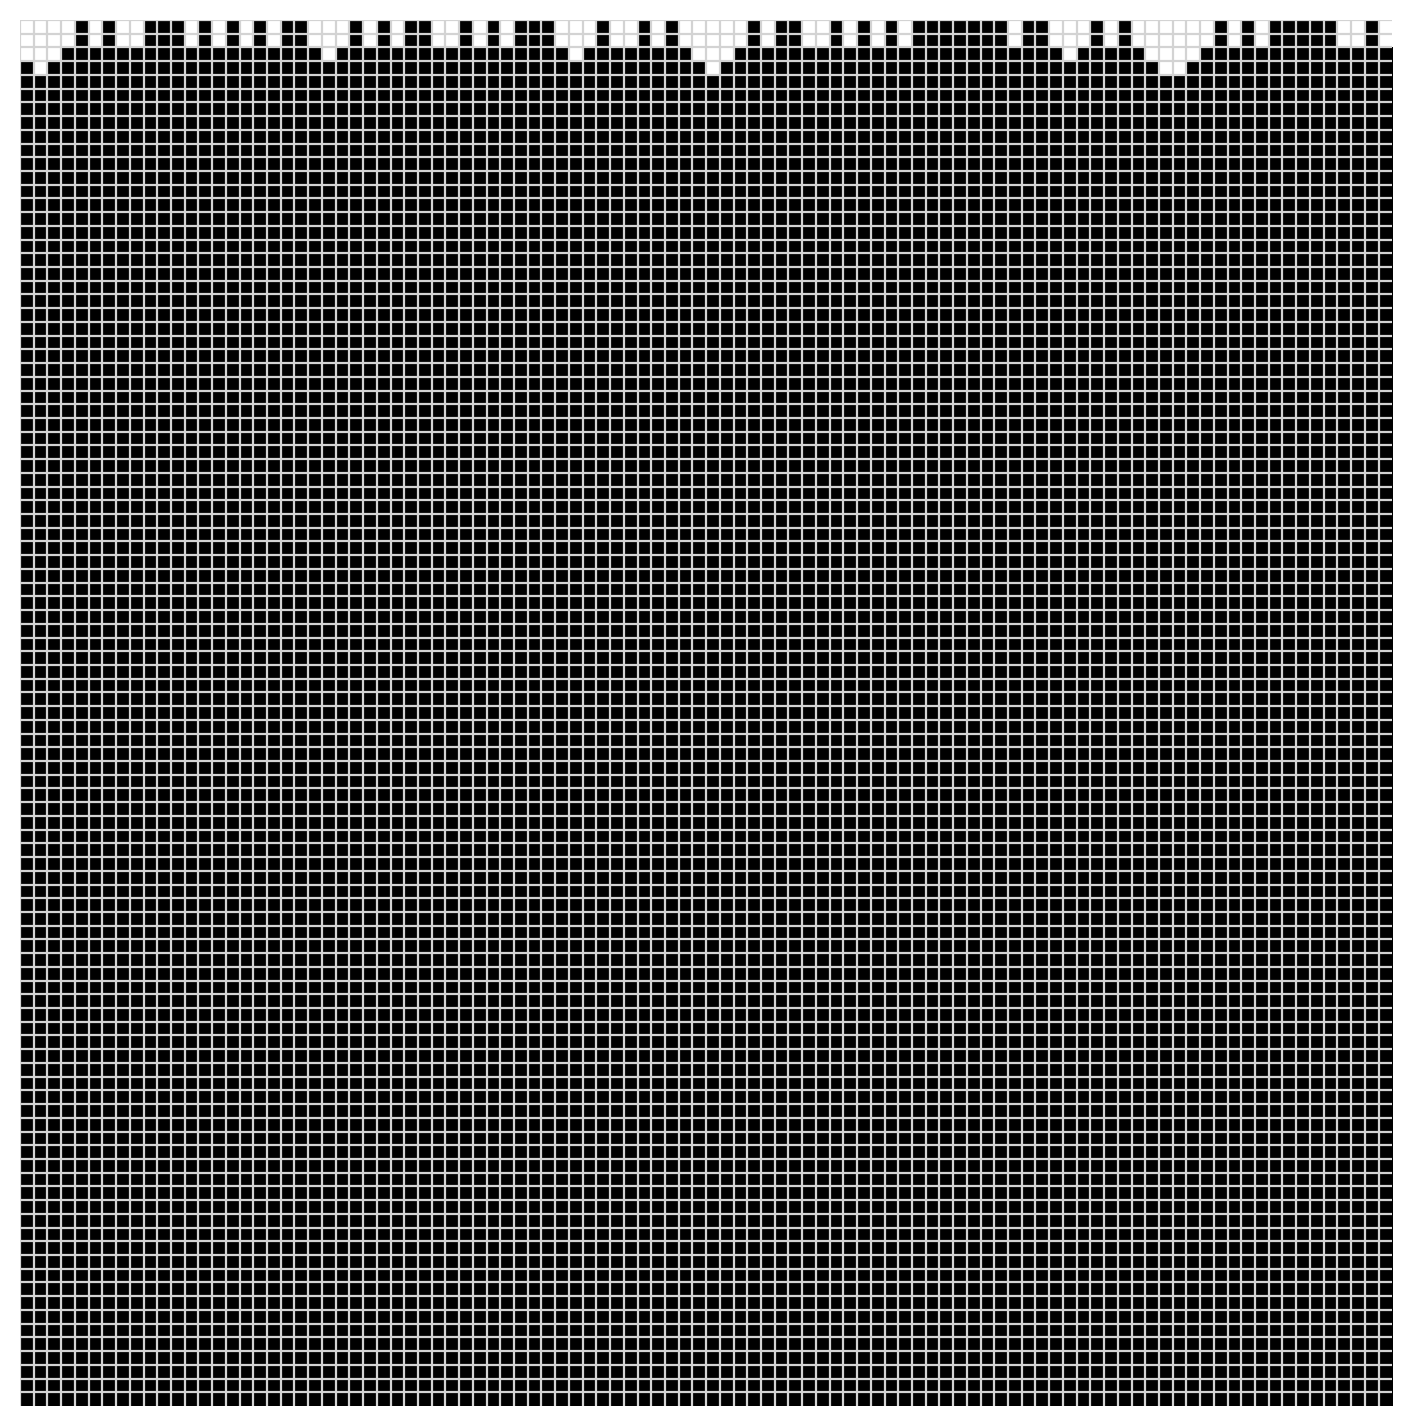
\includegraphics[width=0.2\linewidth]{tarefa-1/rule-254-2.png}
  \caption{Regra $254$.}
\end{figure}

\section{Modelos de crescimento com aleatoriedade}




\section*{Anotações da aula}

- bit de configuracao de uma posicao \( b_i = 0, 1 \) um bit de informacao p/ uma rede/cadeia
\( i = 1, 2, \cdots , L \). 

- configuracao do sistema \( C_t = \{ b_1^t, b_2^2, \cdots , b_L^t\} \) 

- evolucao \( C_{t+1} = f(C_t) \), \( f \rightarrow \) regra de crescimento 
- regra mais simples: \( b_i^{t + 1} = f(b_{i-1}^t, b_i^t, b_{i+1}^t)\) cada posição
depende dos adjacentes.

- Modelo Eden e DLA -> 



\appendix

\clearpage
\section{Regras de 0 à 255}


 %\begin{figure}[htbp]
  \centering

\includegraphics[width=0.2\linewidth]{tarefa-1/all-the-rules/rule-0-centered.png}

\includegraphics[width=0.2\linewidth]{tarefa-1/all-the-rules/rule-0-last.png}

\includegraphics[width=0.2\linewidth]{tarefa-1/all-the-rules/rule-1-centered.png}

\includegraphics[width=0.2\linewidth]{tarefa-1/all-the-rules/rule-1-last.png}
\end{figure}
\begin{figure}[htbp]
  \centering

\includegraphics[width=0.2\linewidth]{tarefa-1/all-the-rules/rule-2-centered.png}

\includegraphics[width=0.2\linewidth]{tarefa-1/all-the-rules/rule-2-last.png}

\includegraphics[width=0.2\linewidth]{tarefa-1/all-the-rules/rule-3-centered.png}

\includegraphics[width=0.2\linewidth]{tarefa-1/all-the-rules/rule-3-last.png}
\end{figure}
\begin{figure}[htbp]
  \centering

\includegraphics[width=0.2\linewidth]{tarefa-1/all-the-rules/rule-4-centered.png}

\includegraphics[width=0.2\linewidth]{tarefa-1/all-the-rules/rule-4-last.png}

\includegraphics[width=0.2\linewidth]{tarefa-1/all-the-rules/rule-5-centered.png}

\includegraphics[width=0.2\linewidth]{tarefa-1/all-the-rules/rule-5-last.png}
\end{figure}
\begin{figure}[htbp]
  \centering

\includegraphics[width=0.2\linewidth]{tarefa-1/all-the-rules/rule-6-centered.png}

\includegraphics[width=0.2\linewidth]{tarefa-1/all-the-rules/rule-6-last.png}

\includegraphics[width=0.2\linewidth]{tarefa-1/all-the-rules/rule-7-centered.png}

\includegraphics[width=0.2\linewidth]{tarefa-1/all-the-rules/rule-7-last.png}
\end{figure}
\begin{figure}[htbp]
  \centering}

\includegraphics[width=0.2\linewidth]{tarefa-1/all-the-rules/rule-8-centered.png}

\includegraphics[width=0.2\linewidth]{tarefa-1/all-the-rules/rule-8-last.png}

\includegraphics[width=0.2\linewidth]{tarefa-1/all-the-rules/rule-9-centered.png}

\includegraphics[width=0.2\linewidth]{tarefa-1/all-the-rules/rule-9-last.png}

\includegraphics[width=0.2\linewidth]{tarefa-1/all-the-rules/rule-10-centered.png}
\end{figure}
\begin{figure}[htbp]
  \centering

\includegraphics[width=0.2\linewidth]{tarefa-1/all-the-rules/rule-10-last.png}

\includegraphics[width=0.2\linewidth]{tarefa-1/all-the-rules/rule-11-centered.png}

\includegraphics[width=0.2\linewidth]{tarefa-1/all-the-rules/rule-11-last.png}

\includegraphics[width=0.2\linewidth]{tarefa-1/all-the-rules/rule-12-centered.png}

\includegraphics[width=0.2\linewidth]{tarefa-1/all-the-rules/rule-12-last.png}

\includegraphics[width=0.2\linewidth]{tarefa-1/all-the-rules/rule-13-centered.png}

\includegraphics[width=0.2\linewidth]{tarefa-1/all-the-rules/rule-13-last.png}

\includegraphics[width=0.2\linewidth]{tarefa-1/all-the-rules/rule-14-centered.png}

\includegraphics[width=0.2\linewidth]{tarefa-1/all-the-rules/rule-14-last.png}
\end{figure}
\begin{figure}[htbp]
  \centering

\includegraphics[width=0.2\linewidth]{tarefa-1/all-the-rules/rule-15-centered.png}

\includegraphics[width=0.2\linewidth]{tarefa-1/all-the-rules/rule-15-last.png}

\includegraphics[width=0.2\linewidth]{tarefa-1/all-the-rules/rule-16-centered.png}

\includegraphics[width=0.2\linewidth]{tarefa-1/all-the-rules/rule-16-last.png}
\end{figure}
\begin{figure}[htbp]
  \centering

\includegraphics[width=0.2\linewidth]{tarefa-1/all-the-rules/rule-17-centered.png}

\includegraphics[width=0.2\linewidth]{tarefa-1/all-the-rules/rule-17-last.png}
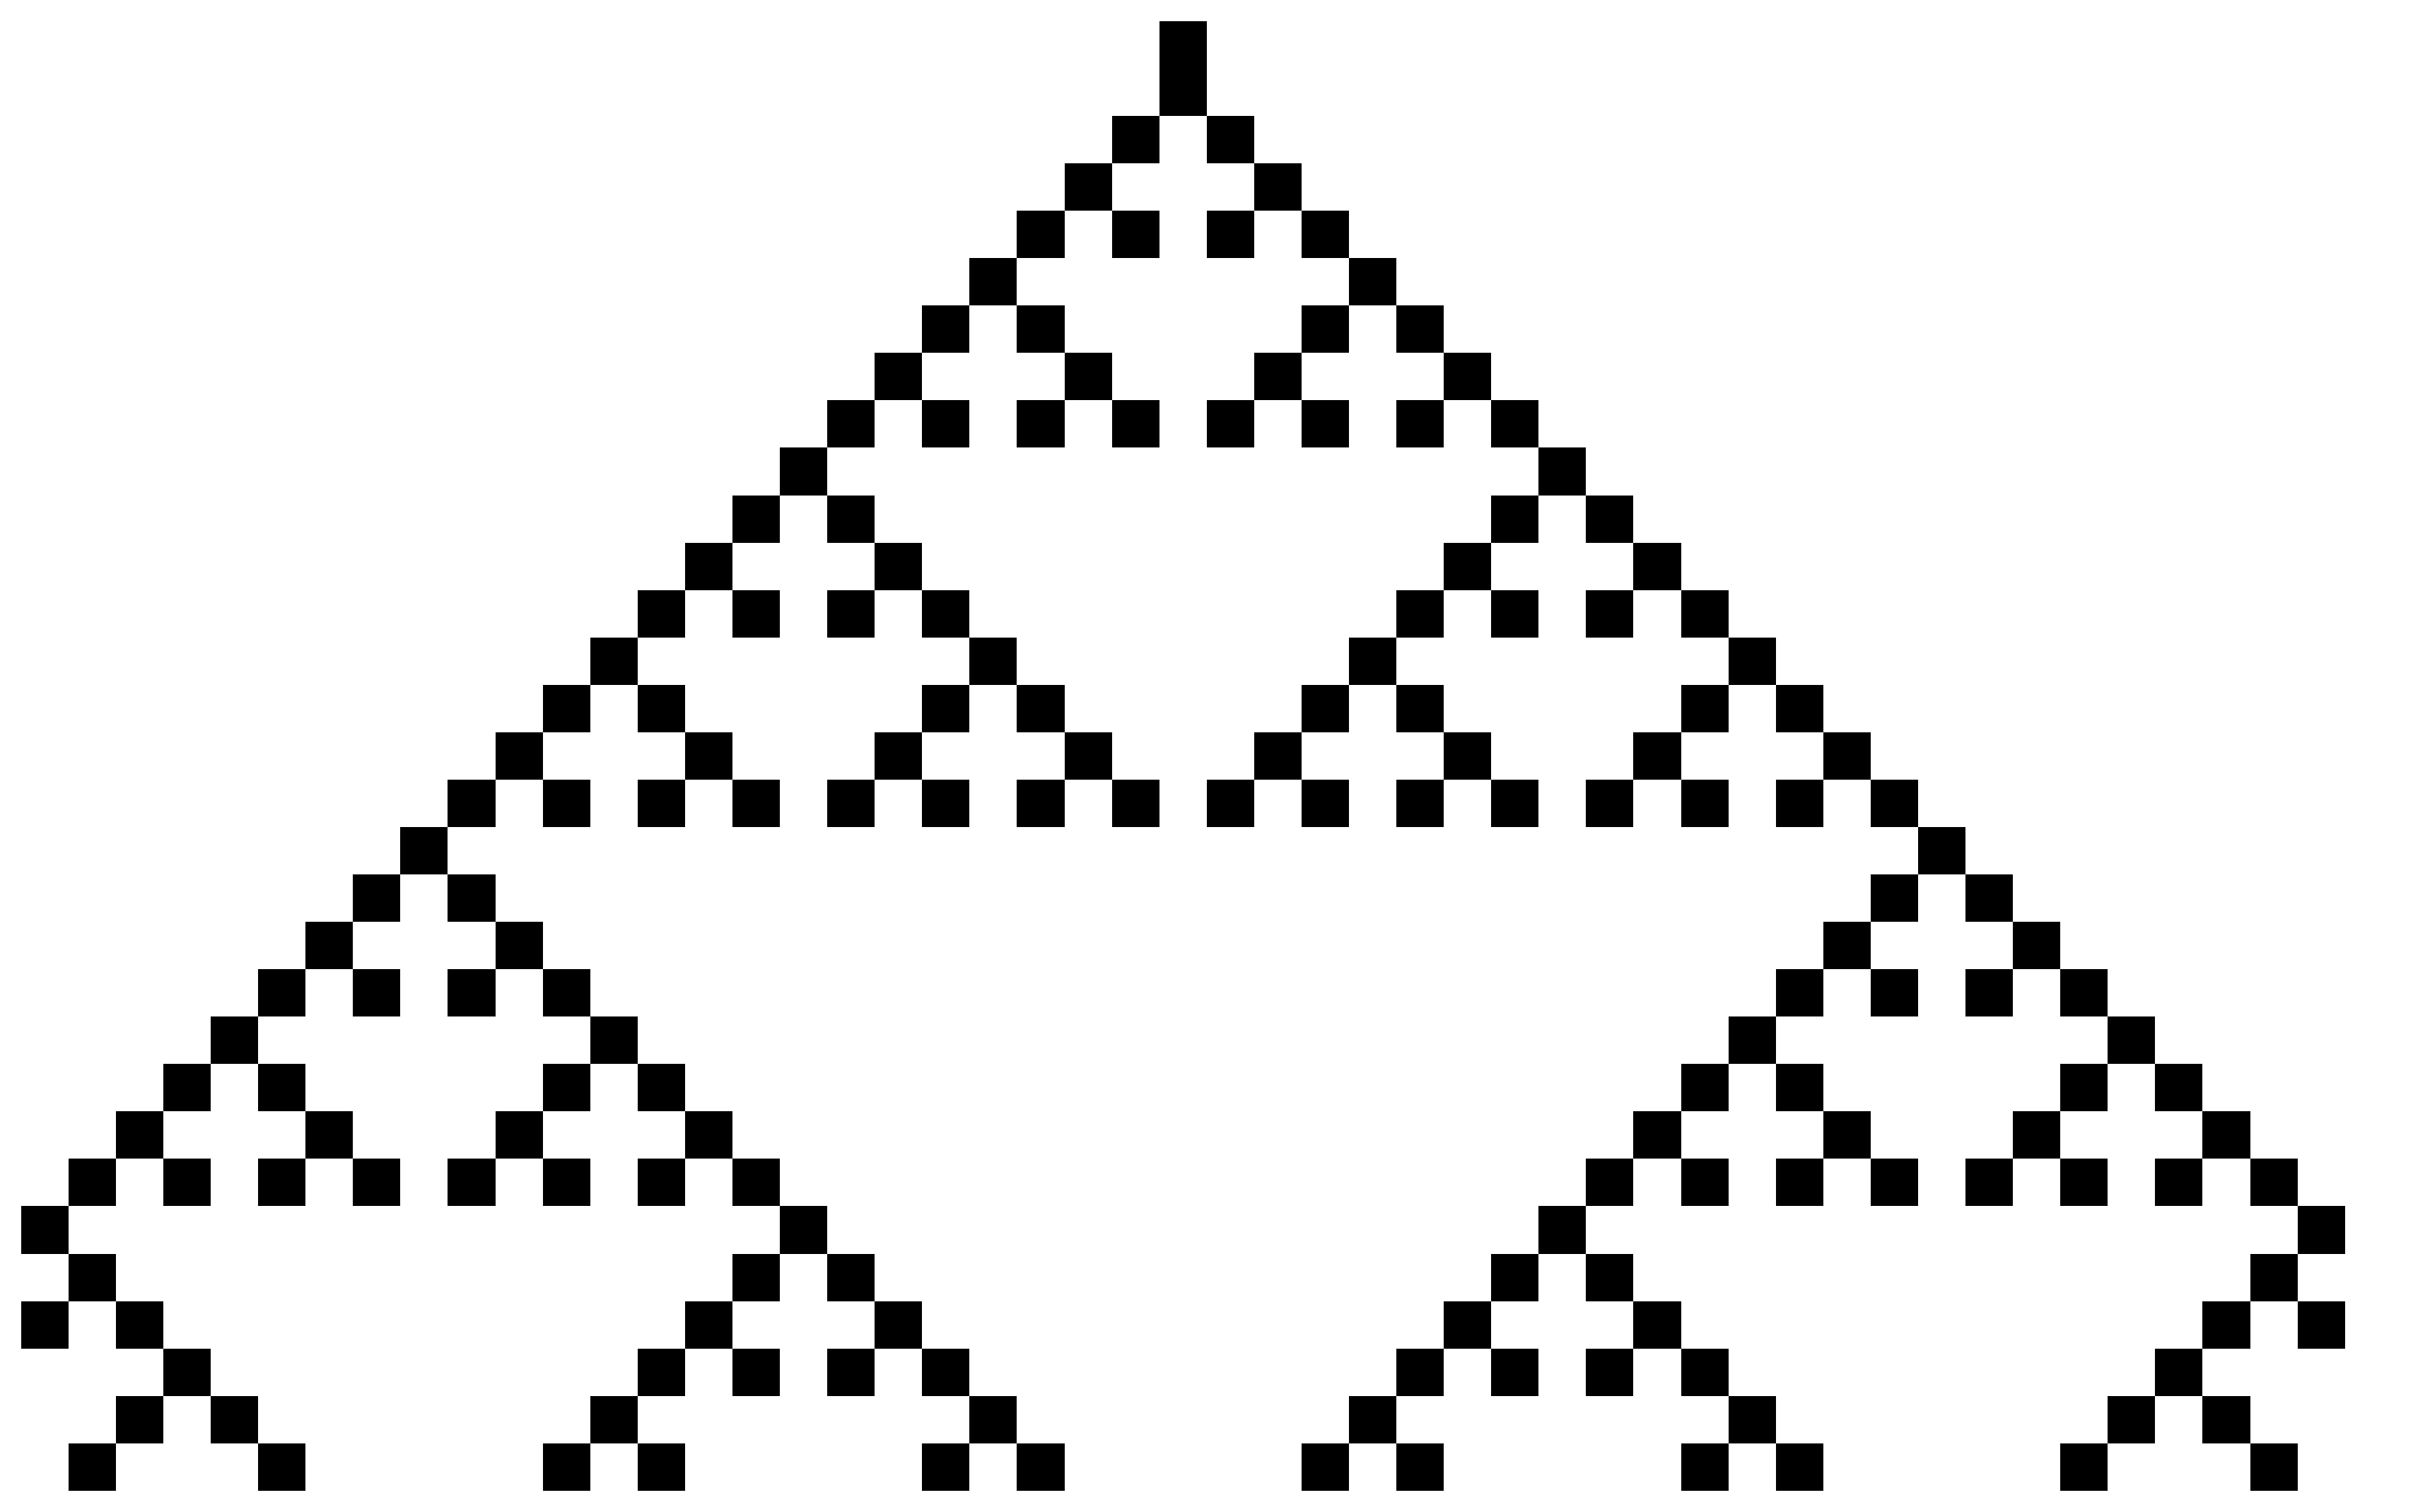
\includegraphics[width=0.2\linewidth]{tarefa-1/all-the-rules/rule-18-centered.png}

\includegraphics[width=0.2\linewidth]{tarefa-1/all-the-rules/rule-18-last.png}
\end{figure}
\begin{figure}[htbp]
  \centering

\includegraphics[width=0.2\linewidth]{tarefa-1/all-the-rules/rule-19-centered.png}

\includegraphics[width=0.2\linewidth]{tarefa-1/all-the-rules/rule-19-last.png}

\includegraphics[width=0.2\linewidth]{tarefa-1/all-the-rules/rule-20-centered.png}
\includegraphics[width=0.2\linewidth]{tarefa-1/all-the-rules/rule-20-last.png}
\end{figure}
\begin{figure}[htbp]
  \centering
\includegraphics[width=0.2\linewidth]{tarefa-1/all-the-rules/rule-21-centered.png}
\includegraphics[width=0.2\linewidth]{tarefa-1/all-the-rules/rule-21-last.png}
\includegraphics[width=0.2\linewidth]{tarefa-1/all-the-rules/rule-22-centered.png}
\includegraphics[width=0.2\linewidth]{tarefa-1/all-the-rules/rule-22-last.png}
\end{figure}
\begin{figure}[htbp]
  \centering
\includegraphics[width=0.2\linewidth]{tarefa-1/all-the-rules/rule-23-centered.png}
\includegraphics[width=0.2\linewidth]{tarefa-1/all-the-rules/rule-23-last.png}
\includegraphics[width=0.2\linewidth]{tarefa-1/all-the-rules/rule-24-centered.png}
\includegraphics[width=0.2\linewidth]{tarefa-1/all-the-rules/rule-24-last.png}
\end{figure}
\begin{figure}[htbp]
  \centering
\includegraphics[width=0.2\linewidth]{tarefa-1/all-the-rules/rule-25-centered.png}
\includegraphics[width=0.2\linewidth]{tarefa-1/all-the-rules/rule-25-last.png}
\includegraphics[width=0.2\linewidth]{tarefa-1/all-the-rules/rule-26-centered.png}
\includegraphics[width=0.2\linewidth]{tarefa-1/all-the-rules/rule-26-last.png}
\end{figure}
\begin{figure}[htbp]
  \centering
\includegraphics[width=0.2\linewidth]{tarefa-1/all-the-rules/rule-27-centered.png}
\includegraphics[width=0.2\linewidth]{tarefa-1/all-the-rules/rule-27-last.png}
\includegraphics[width=0.2\linewidth]{tarefa-1/all-the-rules/rule-28-centered.png}
\includegraphics[width=0.2\linewidth]{tarefa-1/all-the-rules/rule-28-last.png}
\end{figure}
\begin{figure}[htbp]
  \centering
\includegraphics[width=0.2\linewidth]{tarefa-1/all-the-rules/rule-29-centered.png}
\includegraphics[width=0.2\linewidth]{tarefa-1/all-the-rules/rule-29-last.png}
\includegraphics[width=0.2\linewidth]{tarefa-1/all-the-rules/rule-30-centered.png}
\includegraphics[width=0.2\linewidth]{tarefa-1/all-the-rules/rule-30-last.png}
\end{figure}
\begin{figure}[htbp]
  \centering
\includegraphics[width=0.2\linewidth]{tarefa-1/all-the-rules/rule-31-centered.png}
\includegraphics[width=0.2\linewidth]{tarefa-1/all-the-rules/rule-31-last.png}
\includegraphics[width=0.2\linewidth]{tarefa-1/all-the-rules/rule-32-centered.png}
\includegraphics[width=0.2\linewidth]{tarefa-1/all-the-rules/rule-32-last.png}
\end{figure}
\begin{figure}[htbp]
  \centering
\includegraphics[width=0.2\linewidth]{tarefa-1/all-the-rules/rule-33-centered.png}
\includegraphics[width=0.2\linewidth]{tarefa-1/all-the-rules/rule-33-last.png}
\includegraphics[width=0.2\linewidth]{tarefa-1/all-the-rules/rule-34-centered.png}
\includegraphics[width=0.2\linewidth]{tarefa-1/all-the-rules/rule-34-last.png}
\end{figure}
\begin{figure}[htbp]
  \centering
\includegraphics[width=0.2\linewidth]{tarefa-1/all-the-rules/rule-35-centered.png}
\includegraphics[width=0.2\linewidth]{tarefa-1/all-the-rules/rule-35-last.png}
\includegraphics[width=0.2\linewidth]{tarefa-1/all-the-rules/rule-36-centered.png}
\includegraphics[width=0.2\linewidth]{tarefa-1/all-the-rules/rule-36-last.png}
\end{figure}
\begin{figure}[htbp]
  \centering
\includegraphics[width=0.2\linewidth]{tarefa-1/all-the-rules/rule-37-centered.png}
\includegraphics[width=0.2\linewidth]{tarefa-1/all-the-rules/rule-37-last.png}
\includegraphics[width=0.2\linewidth]{tarefa-1/all-the-rules/rule-38-centered.png}
\includegraphics[width=0.2\linewidth]{tarefa-1/all-the-rules/rule-38-last.png}
\end{figure}
\begin{figure}[htbp]
  \centering
\includegraphics[width=0.2\linewidth]{tarefa-1/all-the-rules/rule-39-centered.png}
\includegraphics[width=0.2\linewidth]{tarefa-1/all-the-rules/rule-39-last.png}
\includegraphics[width=0.2\linewidth]{tarefa-1/all-the-rules/rule-40-centered.png}
\includegraphics[width=0.2\linewidth]{tarefa-1/all-the-rules/rule-40-last.png}
\end{figure}
\begin{figure}[htbp]
  \centering
\includegraphics[width=0.2\linewidth]{tarefa-1/all-the-rules/rule-41-centered.png}
\includegraphics[width=0.2\linewidth]{tarefa-1/all-the-rules/rule-41-last.png}
\includegraphics[width=0.2\linewidth]{tarefa-1/all-the-rules/rule-42-centered.png}
\includegraphics[width=0.2\linewidth]{tarefa-1/all-the-rules/rule-42-last.png}
\end{figure}
\begin{figure}[htbp]
  \centering
\includegraphics[width=0.2\linewidth]{tarefa-1/all-the-rules/rule-43-centered.png}
\includegraphics[width=0.2\linewidth]{tarefa-1/all-the-rules/rule-43-last.png}
\includegraphics[width=0.2\linewidth]{tarefa-1/all-the-rules/rule-44-centered.png}
\includegraphics[width=0.2\linewidth]{tarefa-1/all-the-rules/rule-44-last.png}
\end{figure}
\begin{figure}[htbp]
  \centering
\includegraphics[width=0.2\linewidth]{tarefa-1/all-the-rules/rule-45-centered.png}
\includegraphics[width=0.2\linewidth]{tarefa-1/all-the-rules/rule-45-last.png}
\includegraphics[width=0.2\linewidth]{tarefa-1/all-the-rules/rule-46-centered.png}
\includegraphics[width=0.2\linewidth]{tarefa-1/all-the-rules/rule-46-last.png}
\end{figure}
\begin{figure}[htbp]
  \centering
\includegraphics[width=0.2\linewidth]{tarefa-1/all-the-rules/rule-47-centered.png}
\includegraphics[width=0.2\linewidth]{tarefa-1/all-the-rules/rule-47-last.png}
\includegraphics[width=0.2\linewidth]{tarefa-1/all-the-rules/rule-48-centered.png}
\includegraphics[width=0.2\linewidth]{tarefa-1/all-the-rules/rule-48-last.png}
\end{figure}
\begin{figure}[htbp]
  \centering
\includegraphics[width=0.2\linewidth]{tarefa-1/all-the-rules/rule-49-centered.png}
\includegraphics[width=0.2\linewidth]{tarefa-1/all-the-rules/rule-49-last.png}
\includegraphics[width=0.2\linewidth]{tarefa-1/all-the-rules/rule-50-centered.png}
\includegraphics[width=0.2\linewidth]{tarefa-1/all-the-rules/rule-50-last.png}
\end{figure}
\begin{figure}[htbp]
  \centering
\includegraphics[width=0.2\linewidth]{tarefa-1/all-the-rules/rule-51-centered.png}
\includegraphics[width=0.2\linewidth]{tarefa-1/all-the-rules/rule-51-last.png}
\includegraphics[width=0.2\linewidth]{tarefa-1/all-the-rules/rule-52-centered.png}
\includegraphics[width=0.2\linewidth]{tarefa-1/all-the-rules/rule-52-last.png}
\end{figure}
\begin{figure}[htbp]
  \centering
\includegraphics[width=0.2\linewidth]{tarefa-1/all-the-rules/rule-53-centered.png}
\includegraphics[width=0.2\linewidth]{tarefa-1/all-the-rules/rule-53-last.png}
\includegraphics[width=0.2\linewidth]{tarefa-1/all-the-rules/rule-54-centered.png}
\includegraphics[width=0.2\linewidth]{tarefa-1/all-the-rules/rule-54-last.png}
\end{figure}
\begin{figure}[htbp]
  \centering
\includegraphics[width=0.2\linewidth]{tarefa-1/all-the-rules/rule-55-centered.png}
\includegraphics[width=0.2\linewidth]{tarefa-1/all-the-rules/rule-55-last.png}
\includegraphics[width=0.2\linewidth]{tarefa-1/all-the-rules/rule-56-centered.png}
\includegraphics[width=0.2\linewidth]{tarefa-1/all-the-rules/rule-56-last.png}
\end{figure}
\begin{figure}[htbp]
  \centering
\includegraphics[width=0.2\linewidth]{tarefa-1/all-the-rules/rule-57-centered.png}
\includegraphics[width=0.2\linewidth]{tarefa-1/all-the-rules/rule-57-last.png}
\includegraphics[width=0.2\linewidth]{tarefa-1/all-the-rules/rule-58-centered.png}
\includegraphics[width=0.2\linewidth]{tarefa-1/all-the-rules/rule-58-last.png}
\end{figure}
\begin{figure}[htbp]
  \centering
\includegraphics[width=0.2\linewidth]{tarefa-1/all-the-rules/rule-59-centered.png}
\includegraphics[width=0.2\linewidth]{tarefa-1/all-the-rules/rule-59-last.png}
\includegraphics[width=0.2\linewidth]{tarefa-1/all-the-rules/rule-60-centered.png}
\includegraphics[width=0.2\linewidth]{tarefa-1/all-the-rules/rule-60-last.png}
\end{figure}
\begin{figure}[htbp]
  \centering
\includegraphics[width=0.2\linewidth]{tarefa-1/all-the-rules/rule-61-centered.png}
\includegraphics[width=0.2\linewidth]{tarefa-1/all-the-rules/rule-61-last.png}
\includegraphics[width=0.2\linewidth]{tarefa-1/all-the-rules/rule-62-centered.png}
\includegraphics[width=0.2\linewidth]{tarefa-1/all-the-rules/rule-62-last.png}
\end{figure}
\begin{figure}[htbp]
  \centering
\includegraphics[width=0.2\linewidth]{tarefa-1/all-the-rules/rule-63-centered.png}
\includegraphics[width=0.2\linewidth]{tarefa-1/all-the-rules/rule-63-last.png}
\includegraphics[width=0.2\linewidth]{tarefa-1/all-the-rules/rule-64-centered.png}
\includegraphics[width=0.2\linewidth]{tarefa-1/all-the-rules/rule-64-last.png}
\end{figure}
\begin{figure}[htbp]
  \centering
\includegraphics[width=0.2\linewidth]{tarefa-1/all-the-rules/rule-65-centered.png}
\includegraphics[width=0.2\linewidth]{tarefa-1/all-the-rules/rule-65-last.png}
\includegraphics[width=0.2\linewidth]{tarefa-1/all-the-rules/rule-66-centered.png}
\includegraphics[width=0.2\linewidth]{tarefa-1/all-the-rules/rule-66-last.png}
\end{figure}
\begin{figure}[htbp]
  \centering
\includegraphics[width=0.2\linewidth]{tarefa-1/all-the-rules/rule-67-centered.png}
\includegraphics[width=0.2\linewidth]{tarefa-1/all-the-rules/rule-67-last.png}
\includegraphics[width=0.2\linewidth]{tarefa-1/all-the-rules/rule-68-centered.png}
\includegraphics[width=0.2\linewidth]{tarefa-1/all-the-rules/rule-68-last.png}
\end{figure}
\begin{figure}[htbp]
  \centering
\includegraphics[width=0.2\linewidth]{tarefa-1/all-the-rules/rule-69-centered.png}
\includegraphics[width=0.2\linewidth]{tarefa-1/all-the-rules/rule-69-last.png}
\includegraphics[width=0.2\linewidth]{tarefa-1/all-the-rules/rule-70-centered.png}
\includegraphics[width=0.2\linewidth]{tarefa-1/all-the-rules/rule-70-last.png}
\end{figure}
\begin{figure}[htbp]
  \centering
\includegraphics[width=0.2\linewidth]{tarefa-1/all-the-rules/rule-71-centered.png}
\includegraphics[width=0.2\linewidth]{tarefa-1/all-the-rules/rule-71-last.png}
\includegraphics[width=0.2\linewidth]{tarefa-1/all-the-rules/rule-72-centered.png}
\includegraphics[width=0.2\linewidth]{tarefa-1/all-the-rules/rule-72-last.png}
\end{figure}
\begin{figure}[htbp]
  \centering
\includegraphics[width=0.2\linewidth]{tarefa-1/all-the-rules/rule-73-centered.png}
\includegraphics[width=0.2\linewidth]{tarefa-1/all-the-rules/rule-73-last.png}
\includegraphics[width=0.2\linewidth]{tarefa-1/all-the-rules/rule-74-centered.png}
\includegraphics[width=0.2\linewidth]{tarefa-1/all-the-rules/rule-74-last.png}
\end{figure}
\begin{figure}[htbp]
  \centering
\includegraphics[width=0.2\linewidth]{tarefa-1/all-the-rules/rule-75-centered.png}
\includegraphics[width=0.2\linewidth]{tarefa-1/all-the-rules/rule-75-last.png}
\includegraphics[width=0.2\linewidth]{tarefa-1/all-the-rules/rule-76-centered.png}
\includegraphics[width=0.2\linewidth]{tarefa-1/all-the-rules/rule-76-last.png}
\end{figure}
\begin{figure}[htbp]
  \centering
\includegraphics[width=0.2\linewidth]{tarefa-1/all-the-rules/rule-77-centered.png}
\includegraphics[width=0.2\linewidth]{tarefa-1/all-the-rules/rule-77-last.png}
\includegraphics[width=0.2\linewidth]{tarefa-1/all-the-rules/rule-78-centered.png}
\includegraphics[width=0.2\linewidth]{tarefa-1/all-the-rules/rule-78-last.png}
\end{figure}
\begin{figure}[htbp]
  \centering
\includegraphics[width=0.2\linewidth]{tarefa-1/all-the-rules/rule-79-centered.png}
\includegraphics[width=0.2\linewidth]{tarefa-1/all-the-rules/rule-79-last.png}
\includegraphics[width=0.2\linewidth]{tarefa-1/all-the-rules/rule-80-centered.png}
\includegraphics[width=0.2\linewidth]{tarefa-1/all-the-rules/rule-80-last.png}
\end{figure}
\begin{figure}[htbp]
  \centering
\includegraphics[width=0.2\linewidth]{tarefa-1/all-the-rules/rule-81-centered.png}
\includegraphics[width=0.2\linewidth]{tarefa-1/all-the-rules/rule-81-last.png}
\includegraphics[width=0.2\linewidth]{tarefa-1/all-the-rules/rule-82-centered.png}
\includegraphics[width=0.2\linewidth]{tarefa-1/all-the-rules/rule-82-last.png}
\end{figure}
\begin{figure}[htbp]
  \centering
\includegraphics[width=0.2\linewidth]{tarefa-1/all-the-rules/rule-83-centered.png}
\includegraphics[width=0.2\linewidth]{tarefa-1/all-the-rules/rule-83-last.png}
\includegraphics[width=0.2\linewidth]{tarefa-1/all-the-rules/rule-84-centered.png}
\includegraphics[width=0.2\linewidth]{tarefa-1/all-the-rules/rule-84-last.png}
\end{figure}
\begin{figure}[htbp]
  \centering
\includegraphics[width=0.2\linewidth]{tarefa-1/all-the-rules/rule-85-centered.png}
\includegraphics[width=0.2\linewidth]{tarefa-1/all-the-rules/rule-85-last.png}
\includegraphics[width=0.2\linewidth]{tarefa-1/all-the-rules/rule-86-centered.png}
\includegraphics[width=0.2\linewidth]{tarefa-1/all-the-rules/rule-86-last.png}
\end{figure}
\begin{figure}[htbp]
  \centering
\includegraphics[width=0.2\linewidth]{tarefa-1/all-the-rules/rule-87-centered.png}
\includegraphics[width=0.2\linewidth]{tarefa-1/all-the-rules/rule-87-last.png}
\includegraphics[width=0.2\linewidth]{tarefa-1/all-the-rules/rule-88-centered.png}
\includegraphics[width=0.2\linewidth]{tarefa-1/all-the-rules/rule-88-last.png}
\end{figure}
\begin{figure}[htbp]
  \centering
\includegraphics[width=0.2\linewidth]{tarefa-1/all-the-rules/rule-89-centered.png}
\includegraphics[width=0.2\linewidth]{tarefa-1/all-the-rules/rule-89-last.png}
\includegraphics[width=0.2\linewidth]{tarefa-1/all-the-rules/rule-90-centered.png}
\includegraphics[width=0.2\linewidth]{tarefa-1/all-the-rules/rule-90-last.png}
\end{figure}
\begin{figure}[htbp]
  \centering
\includegraphics[width=0.2\linewidth]{tarefa-1/all-the-rules/rule-91-centered.png}
\includegraphics[width=0.2\linewidth]{tarefa-1/all-the-rules/rule-91-last.png}
\includegraphics[width=0.2\linewidth]{tarefa-1/all-the-rules/rule-92-centered.png}
\includegraphics[width=0.2\linewidth]{tarefa-1/all-the-rules/rule-92-last.png}
\end{figure}
\begin{figure}[htbp]
  \centering
\includegraphics[width=0.2\linewidth]{tarefa-1/all-the-rules/rule-93-centered.png}
\includegraphics[width=0.2\linewidth]{tarefa-1/all-the-rules/rule-93-last.png}
\includegraphics[width=0.2\linewidth]{tarefa-1/all-the-rules/rule-94-centered.png}
\includegraphics[width=0.2\linewidth]{tarefa-1/all-the-rules/rule-94-last.png}
\end{figure}
\begin{figure}[htbp]
  \centering
\includegraphics[width=0.2\linewidth]{tarefa-1/all-the-rules/rule-95-centered.png}
\includegraphics[width=0.2\linewidth]{tarefa-1/all-the-rules/rule-95-last.png}
\includegraphics[width=0.2\linewidth]{tarefa-1/all-the-rules/rule-96-centered.png}
\includegraphics[width=0.2\linewidth]{tarefa-1/all-the-rules/rule-96-last.png}
\end{figure}
\begin{figure}[htbp]
  \centering
\includegraphics[width=0.2\linewidth]{tarefa-1/all-the-rules/rule-97-centered.png}
\includegraphics[width=0.2\linewidth]{tarefa-1/all-the-rules/rule-97-last.png}
\includegraphics[width=0.2\linewidth]{tarefa-1/all-the-rules/rule-98-centered.png}
\includegraphics[width=0.2\linewidth]{tarefa-1/all-the-rules/rule-98-last.png}
\end{figure}
\begin{figure}[htbp]
  \centering
\includegraphics[width=0.2\linewidth]{tarefa-1/all-the-rules/rule-99-centered.png}
\includegraphics[width=0.2\linewidth]{tarefa-1/all-the-rules/rule-99-last.png}
\includegraphics[width=0.2\linewidth]{tarefa-1/all-the-rules/rule-100-centered.png}
\includegraphics[width=0.2\linewidth]{tarefa-1/all-the-rules/rule-100-last.png}
\end{figure}
\begin{figure}[htbp]
  \centering
\includegraphics[width=0.2\linewidth]{tarefa-1/all-the-rules/rule-101-centered.png}
\includegraphics[width=0.2\linewidth]{tarefa-1/all-the-rules/rule-101-last.png}
\includegraphics[width=0.2\linewidth]{tarefa-1/all-the-rules/rule-102-centered.png}
\includegraphics[width=0.2\linewidth]{tarefa-1/all-the-rules/rule-102-last.png}
\end{figure}
\begin{figure}[htbp]
  \centering
\includegraphics[width=0.2\linewidth]{tarefa-1/all-the-rules/rule-103-centered.png}
\includegraphics[width=0.2\linewidth]{tarefa-1/all-the-rules/rule-103-last.png}
\includegraphics[width=0.2\linewidth]{tarefa-1/all-the-rules/rule-104-centered.png}
\includegraphics[width=0.2\linewidth]{tarefa-1/all-the-rules/rule-104-last.png}
\end{figure}
\begin{figure}[htbp]
  \centering
\includegraphics[width=0.2\linewidth]{tarefa-1/all-the-rules/rule-105-centered.png}
\includegraphics[width=0.2\linewidth]{tarefa-1/all-the-rules/rule-105-last.png}
\includegraphics[width=0.2\linewidth]{tarefa-1/all-the-rules/rule-106-centered.png}
\includegraphics[width=0.2\linewidth]{tarefa-1/all-the-rules/rule-106-last.png}
\end{figure}
\begin{figure}[htbp]
  \centering
\includegraphics[width=0.2\linewidth]{tarefa-1/all-the-rules/rule-107-centered.png}
\includegraphics[width=0.2\linewidth]{tarefa-1/all-the-rules/rule-107-last.png}
\includegraphics[width=0.2\linewidth]{tarefa-1/all-the-rules/rule-108-centered.png}
\includegraphics[width=0.2\linewidth]{tarefa-1/all-the-rules/rule-108-last.png}
\end{figure}
\begin{figure}[htbp]
  \centering
\includegraphics[width=0.2\linewidth]{tarefa-1/all-the-rules/rule-109-centered.png}
\includegraphics[width=0.2\linewidth]{tarefa-1/all-the-rules/rule-109-last.png}
\includegraphics[width=0.2\linewidth]{tarefa-1/all-the-rules/rule-110-centered.png}
\includegraphics[width=0.2\linewidth]{tarefa-1/all-the-rules/rule-110-last.png}
\end{figure}
\begin{figure}[htbp]
  \centering
\includegraphics[width=0.2\linewidth]{tarefa-1/all-the-rules/rule-111-centered.png}
\includegraphics[width=0.2\linewidth]{tarefa-1/all-the-rules/rule-111-last.png}
\includegraphics[width=0.2\linewidth]{tarefa-1/all-the-rules/rule-112-centered.png}
\includegraphics[width=0.2\linewidth]{tarefa-1/all-the-rules/rule-112-last.png}
\end{figure}
\begin{figure}[htbp]
  \centering
\includegraphics[width=0.2\linewidth]{tarefa-1/all-the-rules/rule-113-centered.png}
\includegraphics[width=0.2\linewidth]{tarefa-1/all-the-rules/rule-113-last.png}
\includegraphics[width=0.2\linewidth]{tarefa-1/all-the-rules/rule-114-centered.png}
\includegraphics[width=0.2\linewidth]{tarefa-1/all-the-rules/rule-114-last.png}
\end{figure}
\begin{figure}[htbp]
  \centering
\includegraphics[width=0.2\linewidth]{tarefa-1/all-the-rules/rule-115-centered.png}
\includegraphics[width=0.2\linewidth]{tarefa-1/all-the-rules/rule-115-last.png}
\includegraphics[width=0.2\linewidth]{tarefa-1/all-the-rules/rule-116-centered.png}
\includegraphics[width=0.2\linewidth]{tarefa-1/all-the-rules/rule-116-last.png}
\end{figure}
\begin{figure}[htbp]
  \centering
\includegraphics[width=0.2\linewidth]{tarefa-1/all-the-rules/rule-117-centered.png}
\includegraphics[width=0.2\linewidth]{tarefa-1/all-the-rules/rule-117-last.png}
\includegraphics[width=0.2\linewidth]{tarefa-1/all-the-rules/rule-118-centered.png}
\includegraphics[width=0.2\linewidth]{tarefa-1/all-the-rules/rule-118-last.png}
\end{figure}
\begin{figure}[htbp]
  \centering
\includegraphics[width=0.2\linewidth]{tarefa-1/all-the-rules/rule-119-centered.png}
\includegraphics[width=0.2\linewidth]{tarefa-1/all-the-rules/rule-119-last.png}
\includegraphics[width=0.2\linewidth]{tarefa-1/all-the-rules/rule-120-centered.png}
\includegraphics[width=0.2\linewidth]{tarefa-1/all-the-rules/rule-120-last.png}
\end{figure}
\begin{figure}[htbp]
  \centering
\includegraphics[width=0.2\linewidth]{tarefa-1/all-the-rules/rule-121-centered.png}
\includegraphics[width=0.2\linewidth]{tarefa-1/all-the-rules/rule-121-last.png}
\includegraphics[width=0.2\linewidth]{tarefa-1/all-the-rules/rule-122-centered.png}
\includegraphics[width=0.2\linewidth]{tarefa-1/all-the-rules/rule-122-last.png}
\end{figure}
\begin{figure}[htbp]
  \centering
\includegraphics[width=0.2\linewidth]{tarefa-1/all-the-rules/rule-123-centered.png}
\includegraphics[width=0.2\linewidth]{tarefa-1/all-the-rules/rule-123-last.png}
\includegraphics[width=0.2\linewidth]{tarefa-1/all-the-rules/rule-124-centered.png}
\includegraphics[width=0.2\linewidth]{tarefa-1/all-the-rules/rule-124-last.png}
\end{figure}
\begin{figure}[htbp]
  \centering
\includegraphics[width=0.2\linewidth]{tarefa-1/all-the-rules/rule-125-centered.png}
\includegraphics[width=0.2\linewidth]{tarefa-1/all-the-rules/rule-125-last.png}
\includegraphics[width=0.2\linewidth]{tarefa-1/all-the-rules/rule-126-centered.png}
\includegraphics[width=0.2\linewidth]{tarefa-1/all-the-rules/rule-126-last.png}
\end{figure}
\begin{figure}[htbp]
  \centering
\includegraphics[width=0.2\linewidth]{tarefa-1/all-the-rules/rule-127-centered.png}
\includegraphics[width=0.2\linewidth]{tarefa-1/all-the-rules/rule-127-last.png}
\includegraphics[width=0.2\linewidth]{tarefa-1/all-the-rules/rule-128-centered.png}
\includegraphics[width=0.2\linewidth]{tarefa-1/all-the-rules/rule-128-last.png}
\end{figure}
\begin{figure}[htbp]
  \centering
\includegraphics[width=0.2\linewidth]{tarefa-1/all-the-rules/rule-129-centered.png}
\includegraphics[width=0.2\linewidth]{tarefa-1/all-the-rules/rule-129-last.png}
\includegraphics[width=0.2\linewidth]{tarefa-1/all-the-rules/rule-130-centered.png}
\includegraphics[width=0.2\linewidth]{tarefa-1/all-the-rules/rule-130-last.png}
\end{figure}
\begin{figure}[htbp]
  \centering
\includegraphics[width=0.2\linewidth]{tarefa-1/all-the-rules/rule-131-centered.png}
\includegraphics[width=0.2\linewidth]{tarefa-1/all-the-rules/rule-131-last.png}
\includegraphics[width=0.2\linewidth]{tarefa-1/all-the-rules/rule-132-centered.png}
\includegraphics[width=0.2\linewidth]{tarefa-1/all-the-rules/rule-132-last.png}
\end{figure}
\begin{figure}[htbp]
  \centering
\includegraphics[width=0.2\linewidth]{tarefa-1/all-the-rules/rule-133-centered.png}
\includegraphics[width=0.2\linewidth]{tarefa-1/all-the-rules/rule-133-last.png}
\includegraphics[width=0.2\linewidth]{tarefa-1/all-the-rules/rule-134-centered.png}
\includegraphics[width=0.2\linewidth]{tarefa-1/all-the-rules/rule-134-last.png}
\end{figure}
\begin{figure}[htbp]
  \centering
\includegraphics[width=0.2\linewidth]{tarefa-1/all-the-rules/rule-135-centered.png}
\includegraphics[width=0.2\linewidth]{tarefa-1/all-the-rules/rule-135-last.png}
\includegraphics[width=0.2\linewidth]{tarefa-1/all-the-rules/rule-136-centered.png}
\includegraphics[width=0.2\linewidth]{tarefa-1/all-the-rules/rule-136-last.png}
\end{figure}
\begin{figure}[htbp]
  \centering
\includegraphics[width=0.2\linewidth]{tarefa-1/all-the-rules/rule-137-centered.png}
\includegraphics[width=0.2\linewidth]{tarefa-1/all-the-rules/rule-137-last.png}
\includegraphics[width=0.2\linewidth]{tarefa-1/all-the-rules/rule-138-centered.png}
\includegraphics[width=0.2\linewidth]{tarefa-1/all-the-rules/rule-138-last.png}
\end{figure}
\begin{figure}[htbp]
  \centering
\includegraphics[width=0.2\linewidth]{tarefa-1/all-the-rules/rule-139-centered.png}
\includegraphics[width=0.2\linewidth]{tarefa-1/all-the-rules/rule-139-last.png}
\includegraphics[width=0.2\linewidth]{tarefa-1/all-the-rules/rule-140-centered.png}
\includegraphics[width=0.2\linewidth]{tarefa-1/all-the-rules/rule-140-last.png}
\end{figure}
\begin{figure}[htbp]
  \centering
\includegraphics[width=0.2\linewidth]{tarefa-1/all-the-rules/rule-141-centered.png}
\includegraphics[width=0.2\linewidth]{tarefa-1/all-the-rules/rule-141-last.png}
\includegraphics[width=0.2\linewidth]{tarefa-1/all-the-rules/rule-142-centered.png}
\includegraphics[width=0.2\linewidth]{tarefa-1/all-the-rules/rule-142-last.png}
\end{figure}
\begin{figure}[htbp]
  \centering
\includegraphics[width=0.2\linewidth]{tarefa-1/all-the-rules/rule-143-centered.png}
\includegraphics[width=0.2\linewidth]{tarefa-1/all-the-rules/rule-143-last.png}
\includegraphics[width=0.2\linewidth]{tarefa-1/all-the-rules/rule-144-centered.png}
\includegraphics[width=0.2\linewidth]{tarefa-1/all-the-rules/rule-144-last.png}
\end{figure}
\begin{figure}[htbp]
  \centering
\includegraphics[width=0.2\linewidth]{tarefa-1/all-the-rules/rule-145-centered.png}
\includegraphics[width=0.2\linewidth]{tarefa-1/all-the-rules/rule-145-last.png}
\includegraphics[width=0.2\linewidth]{tarefa-1/all-the-rules/rule-146-centered.png}
\includegraphics[width=0.2\linewidth]{tarefa-1/all-the-rules/rule-146-last.png}
\end{figure}
\begin{figure}[htbp]
  \centering
\includegraphics[width=0.2\linewidth]{tarefa-1/all-the-rules/rule-147-centered.png}
\includegraphics[width=0.2\linewidth]{tarefa-1/all-the-rules/rule-147-last.png}
\includegraphics[width=0.2\linewidth]{tarefa-1/all-the-rules/rule-148-centered.png}
\includegraphics[width=0.2\linewidth]{tarefa-1/all-the-rules/rule-148-last.png}
\end{figure}
\begin{figure}[htbp]
  \centering
\includegraphics[width=0.2\linewidth]{tarefa-1/all-the-rules/rule-149-centered.png}
\includegraphics[width=0.2\linewidth]{tarefa-1/all-the-rules/rule-149-last.png}
\includegraphics[width=0.2\linewidth]{tarefa-1/all-the-rules/rule-150-centered.png}
\includegraphics[width=0.2\linewidth]{tarefa-1/all-the-rules/rule-150-last.png}
\end{figure}
\begin{figure}[htbp]
  \centering
\includegraphics[width=0.2\linewidth]{tarefa-1/all-the-rules/rule-151-centered.png}
\includegraphics[width=0.2\linewidth]{tarefa-1/all-the-rules/rule-151-last.png}
\includegraphics[width=0.2\linewidth]{tarefa-1/all-the-rules/rule-152-centered.png}
\includegraphics[width=0.2\linewidth]{tarefa-1/all-the-rules/rule-152-last.png}
\end{figure}
\begin{figure}[htbp]
  \centering
\includegraphics[width=0.2\linewidth]{tarefa-1/all-the-rules/rule-153-centered.png}
\includegraphics[width=0.2\linewidth]{tarefa-1/all-the-rules/rule-153-last.png}
\includegraphics[width=0.2\linewidth]{tarefa-1/all-the-rules/rule-154-centered.png}
\includegraphics[width=0.2\linewidth]{tarefa-1/all-the-rules/rule-154-last.png}
\end{figure}
\begin{figure}[htbp]
  \centering
\includegraphics[width=0.2\linewidth]{tarefa-1/all-the-rules/rule-155-centered.png}
\includegraphics[width=0.2\linewidth]{tarefa-1/all-the-rules/rule-155-last.png}
\includegraphics[width=0.2\linewidth]{tarefa-1/all-the-rules/rule-156-centered.png}
\includegraphics[width=0.2\linewidth]{tarefa-1/all-the-rules/rule-156-last.png}
\end{figure}
\begin{figure}[htbp]
  \centering
\includegraphics[width=0.2\linewidth]{tarefa-1/all-the-rules/rule-157-centered.png}
\includegraphics[width=0.2\linewidth]{tarefa-1/all-the-rules/rule-157-last.png}
\includegraphics[width=0.2\linewidth]{tarefa-1/all-the-rules/rule-158-centered.png}
\includegraphics[width=0.2\linewidth]{tarefa-1/all-the-rules/rule-158-last.png}
\end{figure}
\begin{figure}[htbp]
  \centering
\includegraphics[width=0.2\linewidth]{tarefa-1/all-the-rules/rule-159-centered.png}
\includegraphics[width=0.2\linewidth]{tarefa-1/all-the-rules/rule-159-last.png}
\includegraphics[width=0.2\linewidth]{tarefa-1/all-the-rules/rule-160-centered.png}
\includegraphics[width=0.2\linewidth]{tarefa-1/all-the-rules/rule-160-last.png}
\end{figure}
\begin{figure}[htbp]
  \centering
\includegraphics[width=0.2\linewidth]{tarefa-1/all-the-rules/rule-161-centered.png}
\includegraphics[width=0.2\linewidth]{tarefa-1/all-the-rules/rule-161-last.png}
\includegraphics[width=0.2\linewidth]{tarefa-1/all-the-rules/rule-162-centered.png}
\includegraphics[width=0.2\linewidth]{tarefa-1/all-the-rules/rule-162-last.png}
\end{figure}
\begin{figure}[htbp]
  \centering
\includegraphics[width=0.2\linewidth]{tarefa-1/all-the-rules/rule-163-centered.png}
\includegraphics[width=0.2\linewidth]{tarefa-1/all-the-rules/rule-163-last.png}
\includegraphics[width=0.2\linewidth]{tarefa-1/all-the-rules/rule-164-centered.png}
\includegraphics[width=0.2\linewidth]{tarefa-1/all-the-rules/rule-164-last.png}
\end{figure}
\begin{figure}[htbp]
  \centering
\includegraphics[width=0.2\linewidth]{tarefa-1/all-the-rules/rule-165-centered.png}
\includegraphics[width=0.2\linewidth]{tarefa-1/all-the-rules/rule-165-last.png}
\includegraphics[width=0.2\linewidth]{tarefa-1/all-the-rules/rule-166-centered.png}
\includegraphics[width=0.2\linewidth]{tarefa-1/all-the-rules/rule-166-last.png}
\end{figure}
\begin{figure}[htbp]
  \centering
\includegraphics[width=0.2\linewidth]{tarefa-1/all-the-rules/rule-167-centered.png}
\includegraphics[width=0.2\linewidth]{tarefa-1/all-the-rules/rule-167-last.png}
\includegraphics[width=0.2\linewidth]{tarefa-1/all-the-rules/rule-168-centered.png}
\includegraphics[width=0.2\linewidth]{tarefa-1/all-the-rules/rule-168-last.png}
\end{figure}
\begin{figure}[htbp]
  \centering
\includegraphics[width=0.2\linewidth]{tarefa-1/all-the-rules/rule-169-centered.png}
\includegraphics[width=0.2\linewidth]{tarefa-1/all-the-rules/rule-169-last.png}
\includegraphics[width=0.2\linewidth]{tarefa-1/all-the-rules/rule-170-centered.png}
\includegraphics[width=0.2\linewidth]{tarefa-1/all-the-rules/rule-170-last.png}
\end{figure}
\begin{figure}[htbp]
  \centering
\includegraphics[width=0.2\linewidth]{tarefa-1/all-the-rules/rule-171-centered.png}
\includegraphics[width=0.2\linewidth]{tarefa-1/all-the-rules/rule-171-last.png}
\includegraphics[width=0.2\linewidth]{tarefa-1/all-the-rules/rule-172-centered.png}
\includegraphics[width=0.2\linewidth]{tarefa-1/all-the-rules/rule-172-last.png}
\end{figure}
\begin{figure}[htbp]
  \centering
\includegraphics[width=0.2\linewidth]{tarefa-1/all-the-rules/rule-173-centered.png}
\includegraphics[width=0.2\linewidth]{tarefa-1/all-the-rules/rule-173-last.png}
\includegraphics[width=0.2\linewidth]{tarefa-1/all-the-rules/rule-174-centered.png}
\includegraphics[width=0.2\linewidth]{tarefa-1/all-the-rules/rule-174-last.png}
\end{figure}
\begin{figure}[htbp]
  \centering
\includegraphics[width=0.2\linewidth]{tarefa-1/all-the-rules/rule-175-centered.png}
\includegraphics[width=0.2\linewidth]{tarefa-1/all-the-rules/rule-175-last.png}
\includegraphics[width=0.2\linewidth]{tarefa-1/all-the-rules/rule-176-centered.png}
\includegraphics[width=0.2\linewidth]{tarefa-1/all-the-rules/rule-176-last.png}
\end{figure}
\begin{figure}[htbp]
  \centering
\includegraphics[width=0.2\linewidth]{tarefa-1/all-the-rules/rule-177-centered.png}
\includegraphics[width=0.2\linewidth]{tarefa-1/all-the-rules/rule-177-last.png}
\includegraphics[width=0.2\linewidth]{tarefa-1/all-the-rules/rule-178-centered.png}
\includegraphics[width=0.2\linewidth]{tarefa-1/all-the-rules/rule-178-last.png}
\end{figure}
\begin{figure}[htbp]
  \centering
\includegraphics[width=0.2\linewidth]{tarefa-1/all-the-rules/rule-179-centered.png}
\includegraphics[width=0.2\linewidth]{tarefa-1/all-the-rules/rule-179-last.png}
\includegraphics[width=0.2\linewidth]{tarefa-1/all-the-rules/rule-180-centered.png}
\includegraphics[width=0.2\linewidth]{tarefa-1/all-the-rules/rule-180-last.png}
\end{figure}
\begin{figure}[htbp]
  \centering
\includegraphics[width=0.2\linewidth]{tarefa-1/all-the-rules/rule-181-centered.png}
\includegraphics[width=0.2\linewidth]{tarefa-1/all-the-rules/rule-181-last.png}
\includegraphics[width=0.2\linewidth]{tarefa-1/all-the-rules/rule-182-centered.png}
\includegraphics[width=0.2\linewidth]{tarefa-1/all-the-rules/rule-182-last.png}
\end{figure}
\begin{figure}[htbp]
  \centering
\includegraphics[width=0.2\linewidth]{tarefa-1/all-the-rules/rule-183-centered.png}
\includegraphics[width=0.2\linewidth]{tarefa-1/all-the-rules/rule-183-last.png}
\includegraphics[width=0.2\linewidth]{tarefa-1/all-the-rules/rule-184-centered.png}
\includegraphics[width=0.2\linewidth]{tarefa-1/all-the-rules/rule-184-last.png}
\end{figure}
\begin{figure}[htbp]
  \centering
\includegraphics[width=0.2\linewidth]{tarefa-1/all-the-rules/rule-185-centered.png}
\includegraphics[width=0.2\linewidth]{tarefa-1/all-the-rules/rule-185-last.png}
\includegraphics[width=0.2\linewidth]{tarefa-1/all-the-rules/rule-186-centered.png}
\includegraphics[width=0.2\linewidth]{tarefa-1/all-the-rules/rule-186-last.png}
\end{figure}
\begin{figure}[htbp]
  \centering
\includegraphics[width=0.2\linewidth]{tarefa-1/all-the-rules/rule-187-centered.png}
\includegraphics[width=0.2\linewidth]{tarefa-1/all-the-rules/rule-187-last.png}
\includegraphics[width=0.2\linewidth]{tarefa-1/all-the-rules/rule-188-centered.png}
\includegraphics[width=0.2\linewidth]{tarefa-1/all-the-rules/rule-188-last.png}
\end{figure}
\begin{figure}[htbp]
  \centering
\includegraphics[width=0.2\linewidth]{tarefa-1/all-the-rules/rule-189-centered.png}
\includegraphics[width=0.2\linewidth]{tarefa-1/all-the-rules/rule-189-last.png}
\includegraphics[width=0.2\linewidth]{tarefa-1/all-the-rules/rule-190-centered.png}
\includegraphics[width=0.2\linewidth]{tarefa-1/all-the-rules/rule-190-last.png}
\end{figure}
\begin{figure}[htbp]
  \centering
\includegraphics[width=0.2\linewidth]{tarefa-1/all-the-rules/rule-191-centered.png}
\includegraphics[width=0.2\linewidth]{tarefa-1/all-the-rules/rule-191-last.png}
\includegraphics[width=0.2\linewidth]{tarefa-1/all-the-rules/rule-192-centered.png}
\includegraphics[width=0.2\linewidth]{tarefa-1/all-the-rules/rule-192-last.png}
\end{figure}
\begin{figure}[htbp]
  \centering
\includegraphics[width=0.2\linewidth]{tarefa-1/all-the-rules/rule-193-centered.png}
\includegraphics[width=0.2\linewidth]{tarefa-1/all-the-rules/rule-193-last.png}
\includegraphics[width=0.2\linewidth]{tarefa-1/all-the-rules/rule-194-centered.png}
\includegraphics[width=0.2\linewidth]{tarefa-1/all-the-rules/rule-194-last.png}
\end{figure}
\begin{figure}[htbp]
  \centering
\includegraphics[width=0.2\linewidth]{tarefa-1/all-the-rules/rule-195-centered.png}
\includegraphics[width=0.2\linewidth]{tarefa-1/all-the-rules/rule-195-last.png}
\includegraphics[width=0.2\linewidth]{tarefa-1/all-the-rules/rule-196-centered.png}
\includegraphics[width=0.2\linewidth]{tarefa-1/all-the-rules/rule-196-last.png}
\end{figure}
\begin{figure}[htbp]
  \centering
\includegraphics[width=0.2\linewidth]{tarefa-1/all-the-rules/rule-197-centered.png}
\includegraphics[width=0.2\linewidth]{tarefa-1/all-the-rules/rule-197-last.png}
\includegraphics[width=0.2\linewidth]{tarefa-1/all-the-rules/rule-198-centered.png}
\includegraphics[width=0.2\linewidth]{tarefa-1/all-the-rules/rule-198-last.png}
\end{figure}
\begin{figure}[htbp]
  \centering
\includegraphics[width=0.2\linewidth]{tarefa-1/all-the-rules/rule-199-centered.png}
\includegraphics[width=0.2\linewidth]{tarefa-1/all-the-rules/rule-199-last.png}
\includegraphics[width=0.2\linewidth]{tarefa-1/all-the-rules/rule-200-centered.png}
\includegraphics[width=0.2\linewidth]{tarefa-1/all-the-rules/rule-200-last.png}
\end{figure}
\begin{figure}[htbp]
  \centering
\includegraphics[width=0.2\linewidth]{tarefa-1/all-the-rules/rule-201-centered.png}
\includegraphics[width=0.2\linewidth]{tarefa-1/all-the-rules/rule-201-last.png}
\includegraphics[width=0.2\linewidth]{tarefa-1/all-the-rules/rule-202-centered.png}
\includegraphics[width=0.2\linewidth]{tarefa-1/all-the-rules/rule-202-last.png}
\end{figure}
\begin{figure}[htbp]
  \centering
\includegraphics[width=0.2\linewidth]{tarefa-1/all-the-rules/rule-203-centered.png}
\includegraphics[width=0.2\linewidth]{tarefa-1/all-the-rules/rule-203-last.png}
\includegraphics[width=0.2\linewidth]{tarefa-1/all-the-rules/rule-204-centered.png}
\includegraphics[width=0.2\linewidth]{tarefa-1/all-the-rules/rule-204-last.png}
\end{figure}
\begin{figure}[htbp]
  \centering
\includegraphics[width=0.2\linewidth]{tarefa-1/all-the-rules/rule-205-centered.png}
\includegraphics[width=0.2\linewidth]{tarefa-1/all-the-rules/rule-205-last.png}
\includegraphics[width=0.2\linewidth]{tarefa-1/all-the-rules/rule-206-centered.png}
\includegraphics[width=0.2\linewidth]{tarefa-1/all-the-rules/rule-206-last.png}
\end{figure}
\begin{figure}[htbp]
  \centering
\includegraphics[width=0.2\linewidth]{tarefa-1/all-the-rules/rule-207-centered.png}
\includegraphics[width=0.2\linewidth]{tarefa-1/all-the-rules/rule-207-last.png}
\includegraphics[width=0.2\linewidth]{tarefa-1/all-the-rules/rule-208-centered.png}
\includegraphics[width=0.2\linewidth]{tarefa-1/all-the-rules/rule-208-last.png}
\end{figure}
\begin{figure}[htbp]
  \centering
\includegraphics[width=0.2\linewidth]{tarefa-1/all-the-rules/rule-209-centered.png}
\includegraphics[width=0.2\linewidth]{tarefa-1/all-the-rules/rule-209-last.png}
\includegraphics[width=0.2\linewidth]{tarefa-1/all-the-rules/rule-210-centered.png}
\includegraphics[width=0.2\linewidth]{tarefa-1/all-the-rules/rule-210-last.png}
\end{figure}
\begin{figure}[htbp]
  \centering
\includegraphics[width=0.2\linewidth]{tarefa-1/all-the-rules/rule-211-centered.png}
\includegraphics[width=0.2\linewidth]{tarefa-1/all-the-rules/rule-211-last.png}
\includegraphics[width=0.2\linewidth]{tarefa-1/all-the-rules/rule-212-centered.png}
\includegraphics[width=0.2\linewidth]{tarefa-1/all-the-rules/rule-212-last.png}
\end{figure}
\begin{figure}[htbp]
  \centering
\includegraphics[width=0.2\linewidth]{tarefa-1/all-the-rules/rule-213-centered.png}
\includegraphics[width=0.2\linewidth]{tarefa-1/all-the-rules/rule-213-last.png}
\includegraphics[width=0.2\linewidth]{tarefa-1/all-the-rules/rule-214-centered.png}
\includegraphics[width=0.2\linewidth]{tarefa-1/all-the-rules/rule-214-last.png}
\end{figure}
\begin{figure}[htbp]
  \centering
\includegraphics[width=0.2\linewidth]{tarefa-1/all-the-rules/rule-215-centered.png}
\includegraphics[width=0.2\linewidth]{tarefa-1/all-the-rules/rule-215-last.png}
\includegraphics[width=0.2\linewidth]{tarefa-1/all-the-rules/rule-216-centered.png}
\includegraphics[width=0.2\linewidth]{tarefa-1/all-the-rules/rule-216-last.png}
\end{figure}
\begin{figure}[htbp]
  \centering
\includegraphics[width=0.2\linewidth]{tarefa-1/all-the-rules/rule-217-centered.png}
\includegraphics[width=0.2\linewidth]{tarefa-1/all-the-rules/rule-217-last.png}
\includegraphics[width=0.2\linewidth]{tarefa-1/all-the-rules/rule-218-centered.png}
\includegraphics[width=0.2\linewidth]{tarefa-1/all-the-rules/rule-218-last.png}
\end{figure}
\begin{figure}[htbp]
  \centering
\includegraphics[width=0.2\linewidth]{tarefa-1/all-the-rules/rule-219-centered.png}
\includegraphics[width=0.2\linewidth]{tarefa-1/all-the-rules/rule-219-last.png}
\includegraphics[width=0.2\linewidth]{tarefa-1/all-the-rules/rule-220-centered.png}
\includegraphics[width=0.2\linewidth]{tarefa-1/all-the-rules/rule-220-last.png}
\end{figure}
\begin{figure}[htbp]
  \centering
\includegraphics[width=0.2\linewidth]{tarefa-1/all-the-rules/rule-221-centered.png}
\includegraphics[width=0.2\linewidth]{tarefa-1/all-the-rules/rule-221-last.png}
\includegraphics[width=0.2\linewidth]{tarefa-1/all-the-rules/rule-222-centered.png}
\includegraphics[width=0.2\linewidth]{tarefa-1/all-the-rules/rule-222-last.png}
\end{figure}
\begin{figure}[htbp]
  \centering
\includegraphics[width=0.2\linewidth]{tarefa-1/all-the-rules/rule-223-centered.png}
\includegraphics[width=0.2\linewidth]{tarefa-1/all-the-rules/rule-223-last.png}
\includegraphics[width=0.2\linewidth]{tarefa-1/all-the-rules/rule-224-centered.png}
\includegraphics[width=0.2\linewidth]{tarefa-1/all-the-rules/rule-224-last.png}
\end{figure}
\begin{figure}[htbp]
  \centering
\includegraphics[width=0.2\linewidth]{tarefa-1/all-the-rules/rule-225-centered.png}
\includegraphics[width=0.2\linewidth]{tarefa-1/all-the-rules/rule-225-last.png}
\includegraphics[width=0.2\linewidth]{tarefa-1/all-the-rules/rule-226-centered.png}
\includegraphics[width=0.2\linewidth]{tarefa-1/all-the-rules/rule-226-last.png}
\end{figure}
\begin{figure}[htbp]
  \centering
\includegraphics[width=0.2\linewidth]{tarefa-1/all-the-rules/rule-227-centered.png}
\includegraphics[width=0.2\linewidth]{tarefa-1/all-the-rules/rule-227-last.png}
\includegraphics[width=0.2\linewidth]{tarefa-1/all-the-rules/rule-228-centered.png}
\includegraphics[width=0.2\linewidth]{tarefa-1/all-the-rules/rule-228-last.png}
\end{figure}
\begin{figure}[htbp]
  \centering
\includegraphics[width=0.2\linewidth]{tarefa-1/all-the-rules/rule-229-centered.png}
\includegraphics[width=0.2\linewidth]{tarefa-1/all-the-rules/rule-229-last.png}
\includegraphics[width=0.2\linewidth]{tarefa-1/all-the-rules/rule-230-centered.png}
\includegraphics[width=0.2\linewidth]{tarefa-1/all-the-rules/rule-230-last.png}
\end{figure}
\begin{figure}[htbp]
  \centering
\includegraphics[width=0.2\linewidth]{tarefa-1/all-the-rules/rule-231-centered.png}
\includegraphics[width=0.2\linewidth]{tarefa-1/all-the-rules/rule-231-last.png}
\includegraphics[width=0.2\linewidth]{tarefa-1/all-the-rules/rule-232-centered.png}
\includegraphics[width=0.2\linewidth]{tarefa-1/all-the-rules/rule-232-last.png}
\end{figure}
\begin{figure}[htbp]
  \centering
\includegraphics[width=0.2\linewidth]{tarefa-1/all-the-rules/rule-233-centered.png}
\includegraphics[width=0.2\linewidth]{tarefa-1/all-the-rules/rule-233-last.png}
\includegraphics[width=0.2\linewidth]{tarefa-1/all-the-rules/rule-234-centered.png}
\includegraphics[width=0.2\linewidth]{tarefa-1/all-the-rules/rule-234-last.png}
\end{figure}
\begin{figure}[htbp]
  \centering
\includegraphics[width=0.2\linewidth]{tarefa-1/all-the-rules/rule-235-centered.png}
\includegraphics[width=0.2\linewidth]{tarefa-1/all-the-rules/rule-235-last.png}
\includegraphics[width=0.2\linewidth]{tarefa-1/all-the-rules/rule-236-centered.png}
\includegraphics[width=0.2\linewidth]{tarefa-1/all-the-rules/rule-236-last.png}
\end{figure}
\begin{figure}[htbp]
  \centering
\includegraphics[width=0.2\linewidth]{tarefa-1/all-the-rules/rule-237-centered.png}
\includegraphics[width=0.2\linewidth]{tarefa-1/all-the-rules/rule-237-last.png}
\includegraphics[width=0.2\linewidth]{tarefa-1/all-the-rules/rule-238-centered.png}
\includegraphics[width=0.2\linewidth]{tarefa-1/all-the-rules/rule-238-last.png}
\end{figure}
\begin{figure}[htbp]
  \centering
\includegraphics[width=0.2\linewidth]{tarefa-1/all-the-rules/rule-239-centered.png}
\includegraphics[width=0.2\linewidth]{tarefa-1/all-the-rules/rule-239-last.png}
\includegraphics[width=0.2\linewidth]{tarefa-1/all-the-rules/rule-240-centered.png}
\includegraphics[width=0.2\linewidth]{tarefa-1/all-the-rules/rule-240-last.png}
\end{figure}
\begin{figure}[htbp]
  \centering
\includegraphics[width=0.2\linewidth]{tarefa-1/all-the-rules/rule-241-centered.png}
\includegraphics[width=0.2\linewidth]{tarefa-1/all-the-rules/rule-241-last.png}
\includegraphics[width=0.2\linewidth]{tarefa-1/all-the-rules/rule-242-centered.png}
\includegraphics[width=0.2\linewidth]{tarefa-1/all-the-rules/rule-242-last.png}
\end{figure}
\begin{figure}[htbp]
  \centering
\includegraphics[width=0.2\linewidth]{tarefa-1/all-the-rules/rule-243-centered.png}
\includegraphics[width=0.2\linewidth]{tarefa-1/all-the-rules/rule-243-last.png}
\includegraphics[width=0.2\linewidth]{tarefa-1/all-the-rules/rule-244-centered.png}
\includegraphics[width=0.2\linewidth]{tarefa-1/all-the-rules/rule-244-last.png}
\end{figure}
\begin{figure}[htbp]
  \centering
\includegraphics[width=0.2\linewidth]{tarefa-1/all-the-rules/rule-245-centered.png}
\includegraphics[width=0.2\linewidth]{tarefa-1/all-the-rules/rule-245-last.png}
\includegraphics[width=0.2\linewidth]{tarefa-1/all-the-rules/rule-246-centered.png}
\includegraphics[width=0.2\linewidth]{tarefa-1/all-the-rules/rule-246-last.png}
\end{figure}
\begin{figure}[htbp]
  \centering
\includegraphics[width=0.2\linewidth]{tarefa-1/all-the-rules/rule-247-centered.png}
\includegraphics[width=0.2\linewidth]{tarefa-1/all-the-rules/rule-247-last.png}
\includegraphics[width=0.2\linewidth]{tarefa-1/all-the-rules/rule-248-centered.png}
\includegraphics[width=0.2\linewidth]{tarefa-1/all-the-rules/rule-248-last.png}
\end{figure}
\begin{figure}[htbp]
  \centering
\includegraphics[width=0.2\linewidth]{tarefa-1/all-the-rules/rule-249-centered.png}
\includegraphics[width=0.2\linewidth]{tarefa-1/all-the-rules/rule-249-last.png}
\includegraphics[width=0.2\linewidth]{tarefa-1/all-the-rules/rule-250-centered.png}
\includegraphics[width=0.2\linewidth]{tarefa-1/all-the-rules/rule-250-last.png}
\end{figure}
\begin{figure}[htbp]
  \centering
\includegraphics[width=0.2\linewidth]{tarefa-1/all-the-rules/rule-251-centered.png}
\includegraphics[width=0.2\linewidth]{tarefa-1/all-the-rules/rule-251-last.png}
\includegraphics[width=0.2\linewidth]{tarefa-1/all-the-rules/rule-252-centered.png}
\includegraphics[width=0.2\linewidth]{tarefa-1/all-the-rules/rule-252-last.png}
\end{figure}
\begin{figure}[htbp]
  \centering
\includegraphics[width=0.2\linewidth]{tarefa-1/all-the-rules/rule-253-centered.png}
\includegraphics[width=0.2\linewidth]{tarefa-1/all-the-rules/rule-253-last.png}
\includegraphics[width=0.2\linewidth]{tarefa-1/all-the-rules/rule-254-centered.png}
\includegraphics[width=0.2\linewidth]{tarefa-1/all-the-rules/rule-254-last.png}
\end{figure}
\begin{figure}[htbp]
  \centering
\includegraphics[width=0.2\linewidth]{tarefa-1/all-the-rules/rule-255-centered.png}
\includegraphics[width=0.2\linewidth]{tarefa-1/all-the-rules/rule-255-last.png}

\end{figure}


%%% Local Variables:
%%% mode: LaTeX
%%% TeX-master: "main"
%%% End:




\end{document}

%%% Local Variables:
%%% mode: latex
%%% TeX-master: "main.tex"
%%% End:
